\documentclass[12pt,margin=0px]{article}

\usepackage{subcaption}
\usepackage{multirow}
\usepackage{listings}
\usepackage{hhline}
\usepackage{graphicx}
\usepackage{float}
\usepackage{fancyhdr}
\usepackage{amsthm}
\usepackage{amssymb}
\usepackage{amsmath}
\usepackage{makecell}
\usepackage[utf8]{inputenc}
\usepackage[thinlines]{easytable}
\usepackage[table,xcdraw]{xcolor}
\usepackage[normalem]{ulem}
\usepackage[a4paper, margin=1in]{geometry}
\usepackage{enumitem}
\usepackage{xcolor}
\usepackage[magyar]{babel}

\newcommand\ddfrac[2]{\frac{\displaystyle #1}{\displaystyle #2}}
\definecolor{mygray}{rgb}{0.15, 0.15, 0.15}
\newcolumntype{C}[1]{>{\centering\arraybackslash}p{#1}}

\setlist[itemize,1]{label=$\bullet$}
\setlist[itemize,2]{label=$\circ$}
\setlist[itemize,3]{label=$\centerdot$}
\setlist[itemize,4]{label=$\cdot$}

\pagestyle{fancy}

\newcommand\blfootnote[1]{%
  \begingroup
  \renewcommand\thefootnote{}\footnote{#1}%
  \addtocounter{footnote}{-1}%
  \endgroup
}

\renewcommand{\figurename}{ábra}
\newenvironment{tetel}[1]{\paragraph{#1 \\}}{}

\newcommand{\N}{\mathbb{N}}
\newcommand{\Z}{\mathbb{Z}}
\newcommand{\R}{\mathbb{R}}
\newcommand{\Q}{\mathbb{Q}}
\newcommand{\C}{\mathbb{C}}

\makeatletter
\renewcommand\paragraph{%
	\@startsection{paragraph}{4}{0mm}%
	{-\baselineskip}%
	{.5\baselineskip}%
	{\normalfont\normalsize\bfseries}}
\makeatother

% A dokument itt kezdődik
\newcommand\lword[1]{\leavevmode\nobreak\hskip0pt plus\linewidth\penalty50\hskip0pt plus-\linewidth\nobreak #1}
\useunder{\uline}{\ul}{}
\fancyhead{}
\cfoot{19. tétel | \thepage. oldal}

\renewcommand{\headrulewidth}{0pt}
\renewcommand{\footrulewidth}{0.4pt}

\begin{document}
    \thispagestyle{fancy}
    \hyphenation{oddword}
    \uchyph=0

    \begin{center}
        {\Large\bfseries\noindent 19. Adatbázisok optimalizálása és konkurencia kezelése} \\
    \end{center}
    	
	\section*{Az adatbázis-kezelő rendszerek feladata, részei}
	
	Adatbázis-kezelő rendszer alatt olyan számítógépprogramot értünk, mely megvalósítja nagy tömegű adat biztonságos tárolását, gyors lekérdezhetőségét és módosíthatóságát, tipikusan egyszerre	több felhasználó számára.\\
	
	\noindent Az adatbázis-kezelési tevékenységeket két csoportra szokás osztani:
    \begin{itemize}
      \item Adatdefiníciós műveletek.
      \begin{itemize}
        \item A definíciós eszközökkel rendelkező nyelveket összefoglalóan\\ \emph{Data Definition Language (DDL)} nevezzük.
      \end{itemize}
      \item Adatmanipulációs műveletek.
      \begin{itemize}
        \item Az adatok manipulációjára szolgáló nyelveket összefoglalóan\\ \emph{Data Manipulation Language-nek (DML)} nevezzük.
      \end{itemize}
    \end{itemize}
	
	\begin{figure}[H]
		\centering
		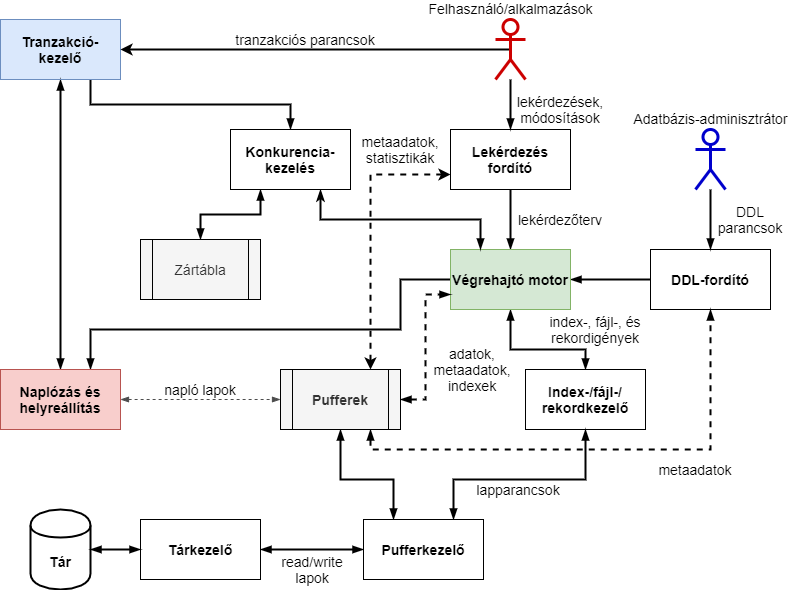
\includegraphics[width=1.0\linewidth]{img/db_felepites}
		\caption{Adatbázis-kezelő rendszer részei.}
		\label{fig:db_felepites}
	\end{figure}
	
	\subsection*{Az egyes alkotórészek rövid jellemzése}

    \begin{itemize}
        \item \textbf{Lekérdezésfordító}: A lekérdezésfordító elemzi és optimalizálja a lekérdezést, ami alapján elkészíti a lekérdezés-végrehajtási tervet (lekérdezéstervet).
        \item \textbf{Végrehajtómotor}: A végrehajtómotor a lekérdezésfordítótól megkapja a lekérdezéstervet, majd kisebb adatdarabokra (tipikusan rekordokra, egy reláció soraira) vonatkozó kérések sorozatát adja át az erőforrás-kezelőnek.
        \item \textbf{Erőforrás-kezelő}: Az erőforrás-kezelő ismeri a relációkat tartalmazó adatfájlokat, a fájlok rekordjainak formátumát, méretét, valamint az indexfájlokat. Az adatkéréseket az erőforrás-kezelő lefordítja lapokra, amit átad a pufferkezelőnek.
        \item \textbf{Pufferkezelő}: Feladata, hogy a másodlagos adattárolóról (lemez, stb.) az adatok megfelelő részét olvassa be a központi memória puffereibe. A pufferkezelő információkat cserél a tárkezelővel, hogy megkapja az adatokat	a lemezről.
	   \item \textbf{Tárkezelő}: Adatokat ír-olvas a másodlagos adattárolóról. Előfordulhat, hogy igénybe veszi az operációs rendszer parancsait is, de sokszor közvetlenül a lemezkezelőhöz intézi a parancsait.
        \item \textbf{Tranzakciókezelő}: A lekérdezéseket és más tevékenységeket tranzakciókba szervezzük. A tranzakciók olyan egységek, amelyeket atomosan és elkülöníthetően kell végrehajtani, valamint a végrehajtásnak tartósnak kell lennie, illetve a tranzakció végrehajtása nem állíthat elő érvénytelen adatbázis-állapotot (azaz konzisztens). A tranzakciókezelő hajtatja végre a tranzakciókat és gondoskodik a naplózásról és helyreállításról, valamint a konkurenciakezelésről.
    \end{itemize}	

    \section*{Fizikai fájlszervezés}

    Az adatbázisban lévő adatokat a memóriában és a háttértárolón tároljuk. A memória és a háttértároló közötti adatávitelért a pufferkezelő modul a felelős. A memória és a háttértároló között átvihető legkisebb egységet \emph{\textbf{blokk}}nak nevezzük.\\\\
    Egy blokk tartalmaz:
    \begin{itemize}
        \item blokk fejlécet
        \item rekordokat
        \item szabad helyet (opcionálisan)
    \end{itemize}
    A blokk-fejlécben általában a blokk sorszámát, a rekordok méretét és azok számát vagy szabad hely kezdetét szokták tárolni.\\

    \noindent Egy rekord mezőkből áll. A relációs adatmodellben például egy adattábla egy sorának egy rekord felel meg, és minden egyes attribútumnak egy mező felel meg. A blokkokhoz hasonlóan a rekordnak is lehet fejléce. Ebben lehet például a\\
    - \emph{rekord sorszáma}, a\\
    - \emph{töröltség jelző flag}, vagy a\\
    - \emph{rekord mérete}.

	\noindent \emph{Jelölések:}\\\\
    \renewcommand{\arraystretch}{1.5}
        \begin{tabular}{ l l l l }
           \hline
           \textit{\textbf{B}}                  & \text{blokk mérete} & \textit{\textbf{R}}                  & \text{rekord mérete}
           \\
           \textit{\textbf{b}}                  & \text{blokkok száma} & \textit{\textbf{r}}                  & \text{rekordok száma}
           \\
           \textit{\textbf{bf}}                 & \textit{blokkolási faktor} & $bf = \lfloor \ddfrac{B}{R} \rfloor$ &
           \\ \hline
        \end{tabular}
    \renewcommand{\arraystretch}{1}\\\\
    \section*{Adatfájlok felépítése}
    A legegyszerűbb adatfájl a rendezetlen fájl, más néven a kupac (heap). Ilyenkor a rekordokat egyszerűen egymás után beírjuk a blokkokba.\\\\
    \renewcommand{\arraystretch}{1.5}
    \begin{tabular}{|l|l|}
       \hline
       \textit{\textbf{Tárigény}}                  & $b=\lceil \ddfrac{r}{bf}\rceil$
       \\ \hline
       \textit{\textbf{Keresés}}                   & $\text{átlagosan}\ \ddfrac{b}{2},\ \text{legrosszabb esetben}\ b$
       \\ \hline
       \textit{\textbf{Beszúrás} (a fájl végére)}  & $1\ \text{olvasás} + 1\ \text{írás}$
       \\ \hline
       \textit{\textbf{Törlés}}                    & $\text{keresés} + 1\ \text{írás (\emph{törölt flag beállítás})}$
       \\ \hline
       \textit{\textbf{Módosítás}}                 & $\text{keresés} + 1\ \text{írás}$
       \\ \hline
    \end{tabular}
    \renewcommand{\arraystretch}{1}\\\\

    \noindent Ha egy mező szerint rendezett fájlt használunk, akkor arra a mezőre vonatkozó keresés meggyorsítható, de cserében a frissítések bonyolultabbak lesznek.\\\\
    \renewcommand{\arraystretch}{1.5}
    \begin{tabular}{|l|l|}
       \hline
       \textit{\textbf{Tárigény}}                  & $b=\lceil \ddfrac{r}{bf}\rceil$
       \\ \hline
       \textit{\textbf{Keresés}}                   & $\log_{2}b,\ \textit{logaritmikus keresés}$
       \\ \hline
       \textit{\textbf{Beszúrás} (a fájl végére)}  & $\text{léptetni kell, átalagosan } \ddfrac{b}{2}\ \text{írás}$
       \\ \hline
       \textit{\textbf{Törlés}}                    & $\text{keresés} + 1\ \text{írás (\emph{törölt flag beállítás})}$
       \\ \hline
       \textit{\textbf{Módosítás}}                 & $\text{keresés} + 1\ \text{írás}$
       \\ \hline
    \end{tabular}
    \renewcommand{\arraystretch}{1}\\\\

    \noindent Az előző nem jó megoldás. A beszúráson javíthatunk úgy, hogy az új rekordokat a fájl végére, egy rendezetlen területre írjuk be. Ekkor a beszúrás műveletigénye csökken. Azonban a fájl végén lévő rendezetlen blokkokat időnként (üresjárati időben, kötegelt feldolgozásban) bele kell illeszteni a rendezett fájlba.\\\\
    \renewcommand{\arraystretch}{1.5}
    \begin{tabular}{|l|l|}
       \hline
       \textit{\textbf{Keresés} ($A=a$ alakú)}       & $\log_{2}b + k,\ \text{ahol \textit{k} a rendezetlen blokkok száma}$
       \\ \hline
       \textit{\textbf{Beszúrás}}                  & $1\ \text{olvasás} + 1\ \text{írás}$
       \\ \hline
       \textit{\textbf{Törlés}}                    & $\text{keresés} + 1\ \text{írás (\emph{törölt flag beállítás})}$
       \\ \hline
       \textit{\textbf{Módosítás}}                 & $\text{keresés} + 1\ \text{írás}$
       \\ \hline
       \textit{\textbf{Karbantartás}}              & $b \log_{2}b\ \text{(\emph{adatbázis újrarendezés})}$
       \\ \hline
    \end{tabular}
    \renewcommand{\arraystretch}{1}\\\\

    \noindent Másik lehetőség a beszúrás javítására, ha üres helyeket hagyunk a blokkokban. Például lehet minden blokk kezdetben csak félig telítve. Ilyenkor szükség van az adatbázis karbantartására. A túltelített blokkokat szétvágni, nehogy teljesen beteljenek.\\\\
    \renewcommand{\arraystretch}{1.15}
    \begin{tabular}{|l|l|}
       \hline
       \textit{\textbf{Tárigény}}                  & $2b$
       \\ \hline
       \textit{\textbf{Keresés} ($A=a$ alakú)}     & $\log_{2}b + 1,\ \textit{logaritmikus keresés}$
       \\ \hline
       \textit{\textbf{Beszúrás}}                  & $\text{keresés} + 1\ \text{írás}$
       \\ \hline
       \textit{\textbf{Törlés}}                    & $\text{keresés} + 1\ \text{írás (\emph{törölt flag beállítás})}$
       \\ \hline
       \textit{\textbf{Módosítás}}                 & $\text{keresés} + 1\ \text{írás}$
       \\ \hline
       \textit{\textbf{Karbantartás}}              & $\text{költséges}$
       \\ \hline
    \end{tabular}
    \renewcommand{\arraystretch}{1}

	\section*{Indexstruktúrák}
	
    Ha tudjuk, hogy egy mező szerint sokat fogunk keresni, akkor az adatbázist a szerint a mező szerint indexeljük. Ha \emph{az adatfájl rendezett}, \emph{\textbf{elsődleges index}ről beszélünk}. Ha az adatfájl \emph{nem rendezett}, vagy egy \emph{másik mezőre készítünk indexet}, akkor azt \textbf{\emph{másodlagos index}}nek nevezzük. Egy index lehet ritka és sűrű index. A ritka indexben csak az egyes blokkok elején lévő kulcsot tüntetjük fel, a sűrű indexben minden értéket. Ritka indexet csak rendezett adatfájlra lehet használni.

	\subsection*{Elsődleges index}
	
    Az elsődleges index olyan mezőre vonatkozik, amelyik szerint az adatfájl rendezett, így csak egy elsődleges index adható meg. Elsődleges indexnek használhatunk ritka indexet. A ritka indexben csak az adatfájl blokkjainak elején lévő kulcs-értékeket tüntetjük fel. Az indexben csak a kulcs-blokkszám párokat kell tárolni, ezért az index rekordmérete is kicsi. Az index rekordjainak száma megegyezik az adatfájl blokkjainak számával.\\\\
    \renewcommand{\arraystretch}{1.15}
    \begin{tabular}{|l|l|}
       \hline
       \textit{\textbf{Tárigény}}                  & $b_{I}=\lceil \ddfrac{b}{bf_{I}} \rceil \ll b$
       \\ \hline
       \textit{\textbf{Keresés} ($A=a$ alakú)}     & $\log_{2}b_{I} + 1$ \text(beolvasás) $\ll \log_{2}b$,\ \textit{logaritmikus keresés}
       \\ \hline
       \textit{\textbf{Frissítések}}               & $\text{bonyolult, ld. rendezett adatfájl}$
       \\ \hline
    \end{tabular}
    \renewcommand{\arraystretch}{1}

	\subsection*{Másodlagos index}
	
    A másodlagos index olyan mezőre vonatkozik, amelyik szerint nincs rendezve az adatfájl. Lehet rendezetlen az adatfájl, vagy lehet, hogy másik mező szerint rendeztük. A másodlagos index egy sűrű index, az adatfájl egyes rekordjához egy index-rekord tartozik. Az index egy rekordjában kulcs-rekord mutató párok vannak.\\\\
    \renewcommand{\arraystretch}{1.15}
    \begin{tabular}{|l|l|}
       \hline
       \textit{\textbf{Tárigény}}                  & $b_{I}=\lceil \ddfrac{r}{bf_{I}} \rceil$
       \\ \hline
       \textit{\textbf{Keresés} ($A=a$ alakú)}     & $\log_{2}b_{I},\ \textit{logaritmikus keresés}$
       \\ \hline
       \textit{\textbf{Frissítések}}               & $\text{bonyolult, ld. rendezett adatfájl}$
       \\ \hline
    \end{tabular}
    \renewcommand{\arraystretch}{1}\\\

    \noindent Az indexek frissítésekor ugyanazok a problémák merülhetnek fel, mint a rendezett \lword{adatfájloknál}. A beszúrás gyorsítására itt is használható részben kitöltött blokk, egy így tovább.

	\subsection*{Bitmap index}
	
	A bitmap indexeket az oszlopok adott értékeihez szokták hozzárendelni, az alábbi módon:
	\begin{itemize}
		\item	Ha az oszlopban az $i$. sor értéke megegyezik az adott értékkel, akkor a bitmap index $i$. tagja
		egy 1-es.	
		
		\item	Ha az oszlopban az $i$. sor értéke viszont nem egyezik meg az adott értékkel, akkor a bitmap
		index $i$. tagja egy 0.
	\end{itemize}

	\noindent Így egy lekérdezésnél csak megfelelően össze kell AND-elni, illetve OR-olni a bitmap indexeket, és az így kapott számsorozatban megkeresni, hol van 1-es. A bináris értékeket szokás szakaszhossz kódolással tömöríteni a hatékonyabb tárolás érdekében.

	\subsection*{Többszintű indexek, keresőfák, B-fák}

    Az index olyan, mint egy rendezett adatfájl, ezért szintén indexelhető elsődleges indexel. Ha az indexet is indexeljük, akkor \emph{\textbf{többszintű indexelés}}ről beszélünk. Mivel az index már rendezett, azt ritka indexel lehet indexelni. Ráadásul az index rekordmérete is kisebb, mint az adattábláé, ezért nagyobb a blokkolási faktora. Ilyenkor az indexek tárigénye növekszik, de a keresés sokkal gyorsabb lesz.\\

    \noindent A $t$. szintű index: az indexszinteket is indexeljük, összesen $t$ szintig.\\
    A $t$. szinten ($I(t)$) bináris kereséssel keressük meg a fedő indexrekordot.\\

    \noindent Követjük a mutatót, minden szinten, és végül a főfájlban: $\log_{2}\Big(B\big(I(t)\big)\Big) + t$ blokkolvasás. Ha a legfelső szint 1 blokkból áll, akkor $t+1$ blokkolvasást jelent. Minden szint blokkolási faktora megegyezik, mert egyforma hosszúak az indexrekordok.\\
	
	\noindent A $t$. szinten 1 blokk: $1=\ddfrac{B}{bf(I)^{t}}$. Azaz $t=\log_{bf(I)}(B) < \log_{2}(B) $, tehát jobb a rendezett fájlszervezésnél.\\

    \noindent A $log_{bf(I)}(B) < \log_{2}\big(B(I)\big) $ is teljesül általában, így az egyszintű indexeknél is gyorsabb.\\

    \renewcommand{\arraystretch}{1.7}
    \noindent \begin{tabular}{|l|l|}
       \hline
       \textit{\textbf{Tárigény}}                  & $b_{1} + b_{2} + \ldots + b_{t}$
       \\ \hline
       \textit{\textbf{Keresés} ($A=a$ alakú)}     & \makecell{$t + \log_{2}b_{t}$,\\ \text{ahol \emph{t} a szintek száma és a legfelső szinten} $b_{t}$\ \text{blokk van}}
       \\ \hline
    \end{tabular}
    \renewcommand{\arraystretch}{1}\\\\

    \noindent Logikailag az index egy rendezett lista. Fizikailag a rendezett sorrendet táblába rendezett mutatók biztosítják.\\

    \noindent A fa struktúrájú indexek B-fákkal ábrázolhatók. A B-fák megoldják a bináris fák kiegyenlítetlenségi problémáját, mivel "alulról" töltjük fel őket. A B-fa egy csomópontjához több kulcsérték tartozhat. A mutatók más csomópontokra mutatnak, és így az összes kulcsértékre az adott csomóponton. Mivel a B-fák kiegyenlítettek (minden ág egyenlő hosszú, vagyis ugyanazon a szinten fejeződik be), kiküszöbölik a változó elérési időket, amik a bináris fákban megfigyelhetők.\\

    \noindent Bár a kulcsértékek és a	hozzájuk kapcsolódó címek még mindig a fa minden szintjén megtalálhatók, és ennek eredménye: egyenlőtlen elérési utak, és egyenlőtlen elérési idő, valamint komplex fakeresési algoritmus az adatfájl logikailag soros olvasására.\\ Ez kiküszöbölhető, ha nem engedjük meg az adatfájl címek tárolását levélszint felett. Ebből következően: minden elérés ugyanolyan hosszú utat vesz igénybe, aminek egyenlő elérési idő az eredménye, és egy logikailag soros olvasása az adatfájlnak a levélszint elérésével megoldható. Nincs szükség komplex fakeresési algoritmusra.\\

    \noindent A B-fa egy csomópontjához több kulcsérték tartozhat. A mutatók más csomópontokra mutatnak, és így az összes kulcsértékre az adott csomóponton. Ilyenkor a keresés \lword{műveletigénye} tovább csökken, bár most is logaritmikus, de a logaritmus alapszáma $bf_{I}$ ritka indexre vonatkozó blokkolási faktor. A módosíthatóság javítására pedig a blokkokban üres helyeket hagyunk. Ezt minden szinten elvégezve a beszúrás, törlés műveletigénye is logaritmikus lesz.\\\\
    \renewcommand{\arraystretch}{1.7}
    \begin{tabular}{|l|l|}
       \hline
       \textit{\textbf{Szintek száma}}             & $t = \log_{bfI} b$
       \\ \hline
       \textit{\textbf{Tárigény}}                  & \text{nagyságrendben lineáris}
       \\ \hline
       \textit{\textbf{Keresés} ($A=a$ alakú)}     & $t + \log_{bfI} b$
       \\ \hline
       \textit{\textbf{Frissítési műveletek}}      & $t + \log_{bfI} b$
       \\ \hline
    \end{tabular}
    \renewcommand{\arraystretch}{1}

	\subsection*{Hasító index}
    \begin{itemize}
    	\item A hasító függvényekkel az A=a alakú kereséseket tudjuk felgyorsítani. A rekordok edényekbe (bucket) particionálva helyezkednek el, melyekre a $h$ hasítómezőn értelmezett függvény osztja szét őket.
        \item Hatékony egyenlőségi keresés, beszúrás, és törlés jellemzi, viszont nem támogatja az intervallumos keresést ($a < A < b$).
    	\item A rekordokat blokkláncokba soroljuk, és a blokklánc utolsó blokkjának első üres helyére tesszük a rekordokat a beérkezés sorrendjében.
        \item A blokkláncok száma lehet
        \begin{itemize}
            \item előre adott (\emph{statikus hasítás}, ekkor a számot $K$-val jelöljük), vagy
            \item a tárolt adatok alapján változhat (\emph{dinamikus hasítás}).
        \end{itemize}
    	\item A besorolás az indexmező értékei alapján történik. Egy $h(x) \in \left\{1,..,K\right\}$ hasító függvény értéke mondja meg,
    	hogy melyik kosárba tartozik a rekord, ha $x$ volt az indexmező értéke a rekordban.
        \item A hasító függvény általában maradékos osztáson alapul (például $mod(K)$).
        \item Akkor jó egy hasító függvény, ha nagyjából egyforma hosszú blokkláncok keletkeznek, azaz egyenletesen sorolja be a rekordokat. Ekkor a blokklánc $\ddfrac{B}{K}$ blokkból áll.
\newpage
    	\item  A keresés költsége (A=a alakú):
        	\begin{itemize}
        		\item	Ha az indexmező és keresési mező eltér, akkor kupac szervezést jelent.
        		\item	Ha az indexmező és keresési mező megegyezik, akkor csak elég a $h(a)$ sorszámú kosarat végignézni,
        		amely $\ddfrac{B}{K}$ blokkból álló kupacnak felel meg, azaz\\
                $\ddfrac{B}{K}$ legrosszabb esetben.
        		A keresés így $K$-szorosára gyorsul.
        	\end{itemize}
    	\item Miért nem érdemes nagy $K$-t választani?
       	   A tárméret $B$, ha minden blokk nagyjából tele van.
            \begin{itemize}
               \item Nagy $K$ esetén sok olyan blokklánc lehet, amely egy blokkból fog állni, és a blokkban is csak 1 rekord lesz. Ekkor a keresési idő: 1 blokkbeolvasás,
        	de $B$ helyett $T$ számú blokkban tároljuk az adatokat.
            \item Módosításnál $\ddfrac{B}{K}$ blokkból álló kupac szervezésű kosarat kell módosítani.
            \end{itemize}
	\end{itemize}

	\section*{Lekérdezések végrehajtása, optimalizálása}
	
	A lekérdezésfeldolgozó egy relációs adatbázis-kezelő komponenseinek azon csoportja, amelyik a felhasználó lekérdezéseit, valamint adatmódosító utasításait lefordítja adatbázis-műveletekre, amiket végre is hajt.
	
    \begin{figure}[H]
        \centering
        $\begin{array}{C{.5\textwidth}C{.5\textwidth}}
            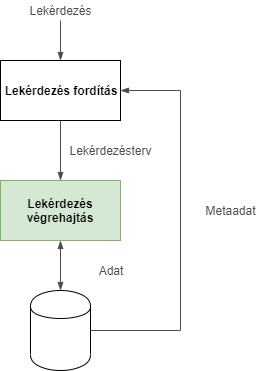
\includegraphics[width=0.75\linewidth]{img/queryprocessing}
            &
            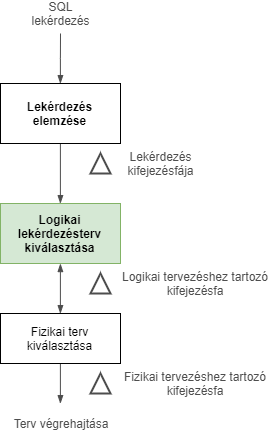
\includegraphics[width=0.75\linewidth]{img/querycompiling}
        \end{array}$
        \caption{A lekérdezésfeldolgozás és lekérdezésfordítás lépései.}
    \end{figure}

	\noindent A lekérdezés végrehajtása tulajdonképpen az adatbázist manipuláló algoritmusok összessége, azonban a végrehajtás előtt szükség van a lekérdezések fordítására.\\
	
	\paragraph*{A lekérdezés-fordítás lépései}
	\begin{enumerate}
		\item	Egy elemző fát építünk fel, amely a lekérdezést és annak szerkezetét jellemzi
		
		\item	Az elemző fából egy kezdeti lekérdezés-tervet készítünk, amelyet átalakítunk
		egy ezzel ekvivalens tervvé, aminek végrehajtási ideje várhatóan kisebb lesz. Elkészül a logikai
		lekérdezésterv, amely relációs algebrai kifejezéseket tartalmaz.
		
		\item	A logikai tervet átalakítjuk fizikai tervvé úgy, hogy a logikai terv operátoraihoz kiválasztunk egy
		algoritmust,  valamint meghatározzuk az operátorok végrehajtási sorrendjét. A fizikai terv olyan részleteket is
		tartalmaz, hogy pl. kell-e rendezni, vagy hogyan férünk hozzá az adatokhoz.
	\end{enumerate}

	\subsection*{Algebrai optimalizálás}
	
    A relációs algebrai kifejezéseket minél gyorsabban akarjuk kiszámolni. A kiszámítás költsége arányos a relációs algebrai kifejezés részkifejezéseinek megfelelő relációk tárolási méreteinek összegével. A módszer az, hogy műveleti tulajdonságokon alapuló ekvivalens átalakításokat alkalmazunk, azért, hogy várhatóan kisebb méretű relációk keletkezzenek.\\

    \noindent Az eljárás heurisztikus, tehát nem az argumentum relációk valódi méretével számol. Az eredmény nem egyértelmű, ugyanis az átalakítások sorrendje nem determinisztikus, így más sorrendben végrehajtva az átalakításokat más végeredményt kaphatunk, de mindegyik általában jobb költségű, mint amiből kiindultunk.\\
	
	\noindent Az optimalizáló algoritmus a következő heurisztikus elveken alapul:
	\begin{itemize}
		\item Minél hamarabb szelektáljunk, hogy a részkifejezések várhatóan kisebb relációk legyenek.
		\item A szorzás utáni kiválasztásokból próbáljunk természetes összekapcsolásokat képezni, mert az összekapcsolás hatékonyabban kiszámolható, mint a szorzatból történő kiválasztás.
        \item Vonjuk össze az egymás utáni unáris műveleteket (kiválasztásokat és vetítéseket), és ezekből lehetőleg egy kiválasztást, vagy vetítést, vagy kiválasztás utáni vetítést képezzünk. Így csökken a műveletek száma, és általában a kiválasztás kisebb relációt eredményez, mint a vetítés.
		\item Keressünk közös részkifejezéseket, amiket így elég csak egyszer kiszámolni a kifejezés kiértékelése során.
	\end{itemize}
\newpage
	\subsection*{Relációs algebrai műveletek megvalósítása}

    \noindent \emph{Jelölések}: $\sigma\ (\textit{szigma}),\ \theta\ (\textit{théta}),\ \pi\ (\textit{pi})$
	
	\subsubsection*{Kiválasztás}
	
	A kiválasztás ($\sigma$) lehetséges megvalósításai:

	\begin{itemize}
		\item	Lineáris keresés: Olvassunk be minden lapot és keressük az egyezéseket (egyenlőség vizsgálat esetén).
		Az átlagos költség a lapok száma, ha a mező nem kulcs, illetve a lapok számának fele, ha a mező kulcs.
		\item	Bináris (logaritmikus) keresés: Csak rendezett mező esetén használható.
		\item	Elsődleges index használata.
		\item	Másodlagos index használata.
	\end{itemize}

	\noindent \textbf{Összetett kiválasztás}
    Előfordulhat, hogy több feltétel van, amelyek és/vagy kapcsolatban vannak egymással. Ennek lehetséges megvalósításai a következők.
	\begin{itemize}
		\item	Konjunkciós kiválasztás esetén ($\sigma_{\theta_{1} \wedge ... \wedge \theta_{n}}$):
		\begin{itemize}
			\item	Válasszuk ki a legkisebb költségű $\sigma_{\theta_{i}}$-t, és azt végezzük el (lásd fent),
			majd az eredményt szűrjük a többi feltételre. \\
            \emph{Költség}: Az egyszerű kiválasztás költsége lesz a kiválasztott $\sigma_{\theta_{i}}$-re.
			
			\item	Ha mindegyik $\theta_{i}$ mezőjére van indexünk, akkor keressük az indexekben és adjuk vissza a megfelelő
			sorok rowid-jeit. Végül vegyük ezek \emph{\textbf{metszetét}}. \\
            \emph{Költség}: az indexekben való keresés összköltsége + a rekordok beolvasása.
		\end{itemize}
		
		\item	Diszjunkciós kiválasztás esetén ($\sigma_{\theta_{1} \vee ... \vee \theta_{n}}$):
		\begin{itemize}
			\item	Lineáris keresés.
				
			\item	Ha mindegyik $\theta_{i}$ mezőjére van indexünk, akkor keressük az indexekben és adjuk vissza a megfelelő
			sorok rowid-jeit. Végül vegyük ezek \emph{\textbf{unióját}}. \\
            \emph{Költség}: az indexekben való keresés összköltsége + a rekordok beolvasása.
			\end{itemize}
	\end{itemize}
	
	\subsection*{Vetítés és halmazműveletek}
	
	Vetítésnél és halmazműveleteknél a duplikátumokat ki kell szűrni.\\
	
	\noindent \textbf{Vetítés ($\pi$) megvalósítása}:
	
	\begin{enumerate}
		\item	Kezdeti átnézés: eldobjuk a felesleges mezőket.
		\item	Duplikátumok törlése: ehhez az eredményt rendezzük az összes mező szerint, így a duplikáltak szomszédosak
		lesznek. Ezeket kell eldobni.
	\end{enumerate}
	
	\noindent A költség a kezdeti átnézés, a rendezés és a duplikátumok törlésének összköltsége lesz.

	\subsection*{Összekapcsolások}
	
	\subsubsection*{Beágyazott ciklusú összekapcsolás (nested loop join) ($R \bowtie_{Z} S$)}
        Bármekkora méretű relációra használható, nem szükséges, hogy az egyik reláció elférjen a memóriában. Két fajtája van, a \emph{sor} és a \emph{blokk} alapú.
		\begin{itemize}
			\item	\textbf{Sor alapú beágyazott ciklusú összekapcsolás}
            \begin{itemize}
            \item Legyen $R$ és $S$ a két összekapcsolandó reláció
            \begin{itemize}
                \item $S$ belső reláció (kisebb méretű)
                \item $R$ külső reláció
            \end{itemize}
            \item Az algoritmus a következő: \\\\
                {\small
                $\begin{array}{llll}
                   \multicolumn{2}{l}{\textbf{R}\ \text{minden}\ t_{R}\ \text{rekordján}} & &  \\
                   & \multicolumn{2}{l}{\textbf{S}\ \text{minden}\ t_{S}\ \text{rekordján}} & \\
                   & & \multicolumn{2}{l}{\text{ha}\ (t_{R}\ \text{egyezik}\ t_{S}\ Z-n)\quad t_{R}.t_{S}\ \text{kiírása}} \\
                   & \text{vége} & &  \\
                  \text{vége} & & & \\
                \end{array}$}\\
            \item Költség:
                \begin{itemize}
                    \item Jó esetben $S$ belefér a memóriába, ekkor csak egyszer kell beolvasni $S$-t, majd mindvégig a memóriában tarthatjuk.\\
                        Ebben az esetben mindkét reláció lapjait egyszer kell beolvasni: $B_R + B_S$
                    \item Legrosszabb esetben mindkét relációból csak egy-egy lap fér bele a memóriába.\\
                        Ekkor $R$ \emph{minden egyes soránál} végig kell olvasni $S$-t: $N_R * B_S + B_R$.
                \end{itemize}
			\end{itemize}
			\item	\textbf{Blokk alapú beágyazott ciklusú összekapcsolás}
            \begin{itemize}

            \item Az algoritmus a következő: \\\\
                {\small
                $\begin{array}{llllll}
                    \multicolumn{2}{l}{\textbf{R}\ \text{minden}\ X_{R}\ \text{lapján}} & & & & \\
                   & \multicolumn{2}{l}{\textbf{S}\ \text{minden}\ X_{S}\ \text{lapján}} & & & \\
                   & & \multicolumn{2}{l}{\textbf{R}\ \text{minden}\ t_{R}\ \text{rekordján}} & & \\
                   & & & \multicolumn{2}{l}{\textbf{S}\ \text{minden}\ t_{S}\ \text{rekordján}} & \\
                   & & & & \multicolumn{2}{l}{\text{ha}\ (t_{R}\ \text{egyezik}\ t_{S}\ Z-n)\ t_{R}.t_{S}\ \text{kiírása}} \\
                   & & & \text{vége} & & \\
                   & & \text{vége} & & & \\
                   & \text{vége} & & & & \\
                  \text{vége} & & & & & \\
                \end{array}$}\\
                \item Költség:
                \begin{itemize}
                    \item Jó esetben $S$ belefér a memóriába, ekkor csak egyszer kell beolvasni $S$-t, majd mindvégig a memóriában tarthatjuk.\\
                        Ebben az esetben mindkét reláció lapjait egyszer kell beolvasni: $B_R + B_S$
                    \item Legrosszabb esetben mindkét relációból csak egy-egy lap fér bele a memóriába.\\
                        Ekkor $R$ \emph{minden egyes lapjánál} végig kell olvasni $S$-t: $B_R * B_S + B_R$.
                \end{itemize}
            \end{itemize}
		\end{itemize}

	\subsubsection*{Összefésüléses rendező összekapcsolás (merge join)}
        \begin{itemize}
            \item A relációk az összekapcsolási mezők szerint rendezettek.
            \item Egyesítjük a rendezett relációkat:
            \begin{itemize}
                \item mutatók az első rekordra mindkét relációban
                \item beolvasunk $S$-ből egy rekordcsoportot, ahol az összekapcsolási attribútum értéke megegyezik
                \item beolvasunk rekordokat $R$-ből és feldolgozzuk.
            \end{itemize}
            \item A rendezett relációkat csak egyszer kell végigolvasni
            \begin{itemize}
                \item Összekapcsolás költsége:\\
                rendezés költsége + $B_s + B_R$ (a két reláció lapjainak száma).
            \end{itemize}
        \end{itemize}

	\subsubsection*{Hasításos összekapcsolás (hash join)}
        \begin{itemize}
            \item Az összekapcsolási attribútumot használjunk hasítókulcsként, és felosztjuk a rekordokat a memóriába elférő részekre
            \begin{itemize}
                \item $R$ rekordjainak felosztása $R_0\ldots R_n-1$
                \item $S$ rekordjainak felosztása $S_0\ldots S_n-1$
            \end{itemize}
            \item Ez után az egymáshoz rendelt kosárpárokat összekapcsoljuk blokk alapú beágyazott ciklusú összekapcsolással, hasítófüggvény alapú indexet használva.
            \begin{itemize}
                \item Összekapcsolás költsége: $2 * (B_R + B_S) + (B_R + B_S)$
            \end{itemize}
        \end{itemize}
	
	\subsubsection*{Több tábla összekapcsolása}

    Az összekapcsolások kommutatívak és asszociatívak, ezért az eredmény szempontjából mindegy, hogy milyen sorrendben kapcsoljuk össze őket. A sorrend viszont befolyásolhatja a hatékonyságot, ugyanis rossz választás esetén a köztes eredmények nagy méretűek lesznek.\\
	
	\noindent A legjobb összekapcsolási fa megtalálása $n$ reláció egy halmazához:
	\begin{itemize}
		\item	Hogy megtaláljuk a legjobb összekapcsolási fát $n$ reláció egy $S$ halmazához,
		vegyük az összes lehetséges tervet mely így néz ki: $S_{1} \Join (S - S_{1})$, ahol $S_{1}$ az $S$ tetszőleges nem üres részhalmaza.
		
		\item	Rekurzívan számítsuk ki $S$ részhalmazainak összekapcsolásának költségeit, hogy meghatározzuk minden egyes terv költségét. Válasszuk a legolcsóbbat.
		
		\item	Mikor bármely részhalmaz terve kiszámításra került, az újbóli kiszámítás helyett tároljuk el és hasznosítsuk újra amikor ismét szükség lesz rá.
	\end{itemize}
	
	\section*{Tranzakciókezelés}
	
	\noindent \textbf{Konzisztens adatbázis}: Az adatbázisokra különböző megszorítások adhatók meg. Az adatbázis konzisztens állapotban
	van, ha kielégíti az összes ilyen megszorítást. Konzisztens adatbázis egy olyan adatbázis, amely konzisztens állapotban van.\\
	
	\noindent A konzisztencia sérülhet a következő esetekben:
	\begin{itemize}
		\item	Tranzakcióhiba: hibásan megírt, rosszul ütemezett, félbehagyott tranzakciók.
		\item	Adatbázis--kezelési hiba: az adatbázis-kezelő valamelyik komponense nem, vagy rosszul hajtja végre a feladatát.
		\item	Hardverhiba: elvész egy adat, vagy megváltozik az értéke.
		\item	Adatmegosztásból származó hiba.
	\end{itemize}
	
	\noindent \textbf{Tranzakció}: Konzisztenciát tartó adatbázis-műveletek sorozata.\\
    Ezek után mindig feltesszük, hogy ha a $T$ tranzakció indulásakor az adatbázis konzisztens állapotban van, akkor ha $T$ egyedül fut le, az adatbázis konzisztens állapotban lesz a futás végén (közben kialakulhat inkonzisztens állapot).\\

	\noindent \emph{Helyesség feltétele}:
	\begin{itemize}
		\item	Ha leáll egy vagy több tranzakció (abort, vagy hiba miatt), akkor is konzisztens adatbázist kapunk.
		\item	Minden egyes tranzakció induláskor konzisztens adatbázist lát.
	\end{itemize}
	
	\noindent A tranzakcióktól a következő tulajdonságokat szoktuk elvárni (ACID):
	
	\begin{itemize}
		\item	Atomosság (\textbf{A}, azaz \emph{Atomicity}): a tranzakció "mindent vagy semmit" jellegű \lword{végrehajtása} (vagy teljesen végrehajtjuk, vagy egyáltalán nem hajtjuk végre).
		\item	Konzisztencia (\textbf{C}, azaz \emph{Consistency}): az a feltétel, hogy a tranzakció megőrizze az adatbázis konzisztenciáját, azaz a tranzakció végrehajtása után is teljesüljenek az adatbázisban előírt konzisztenciamegszorítások.
		\item	Elkülönítés (\textbf{I}, azaz \emph{Isolation}): az a tény, hogy minden tranzakciónak látszólag úgy kell lefutnia, mintha ez alatt az idő alatt semmilyen másik tranzakciót sem hajtanánk végre.
		\item	Tartósság (\textbf{D}, azaz \emph{Durability}): az a feltétel, hogy ha egyszer egy tranzakció befejeződött, akkor már soha többé nem veszhet el a tranzakciónak az adatbázison kifejtett hatása.	
	\end{itemize}
    A konzisztenciát mindig adottnak tekintjük. A másik három tulajdonságot viszont az adatbázis-kezelő rendszernek kell biztosítania, de ettől időnként eltekintünk. Feltesszük, hogy az adatbázis adategységekből, elemekből áll. Az adatbáziselem a fizikai adatbázisban tárolt adatok egyfajta funkcionális egysége, amelynek értékét tranzakciókkal lehet elérni (kiolvasni) vagy módosítani (kiírni). Adatbáziselem pl. a reláció, relációsor, lap.
	
	\subsection*{A tranzakciók alaptevékenységei}
	
	\noindent A tranzakció és az adatbázis kölcsönhatásának három fontos helyszíne van:
	\begin{itemize}
		\item	Az adatbázis elemeit tartalmazó lemezblokkok területe.
		\item	A pufferkezelő által használt virtuális vagy valós memóriaterület.
		\item	A tranzakció memóriaterülete.
	\end{itemize}
	
    \noindent Ahhoz, hogy a tranzakció egy adatbáziselemet beolvashasson, azt előbb memóriapuffer(ek)be kell hozni, ha még nincs ott. Ezt követően tudja a puffer(ek) tartalmát a tranzakció saját memóriaterületére beolvasni.\\

    \noindent Az adatbáziselem új értékének kiírás fordítva történik: előbb a tranzakció kialakítja az új értéket saját memóriaterületén, majd ez az érték másolódik át a megfelelő puffer(ek)be.\\

    \noindent A pufferek tartalmának lemezre írásáról a pufferkezelő dönt. Vagy azonnal lemezre írja a változásokat, vagy nem.\\
	
	\noindent A naplózási algoritmusok és más tranzakciókezelő algoritmusok tanulmányozása során különböző jelölésekre lesz szükség, melyekkel a különböző területek közötti adatmozgásokat írhatjuk le.\\\\
    \noindent A következő alapműveletek használjuk:
	\begin{itemize}
		\item	$INPUT(X)$:
        \begin{itemize}
            \item Az $X$ adatbáziselemet tartalmazó lemezblokk másolása a pufferbe.
        \end{itemize}
		\item	$READ(X,t)$:
        \begin{itemize}
            \item Az X adatbáziselem bemásolása a tranzakció $t$ lokális változójába.
            \item Ha az $X$-et tartalmazó blokk még nincs a memóriában, akkor $INPUT(X)$-et is beleértjük.
        \end{itemize}
		\item	$WRITE(X,t)$:
        \begin{itemize}
            \item A $t$ lokális változó tartalmaz az $X$ adatbáziselem memóriapufferbeli tartalmába másolódik.
            \item Ha az $X$-et tartalmazó blokk még nincs a pufferben, akkor előbb $INPUT(X)$ is végrehajtódik.
        \end{itemize}
		\item	$OUTPUT(X)$:
        \begin{itemize}
            \item Az $X$ adatbáziselemet tartalmazó blokk kiírása lemezre.
        \end{itemize}
	\end{itemize}

	\noindent A továbbiakban feltételezzük, hogy egy adatbáziselem nem nagyobb egy blokknál.
	
	\subsection*{Naplózás és helyreállítás}
	
	Az adatokat meg kell védeni a rendszerhibáktól, ezért szükség van az adatok helyreállíthatóságára. Erre az elsődleges technika a naplózás, amely valamilyen biztonságos módszerrel rögzíti az adatbázisban végrehajtott módosítások történetét.\\
	
	\noindent A napló (log) nem más, mint naplóbejegyzések (log records) sorozata, melyek arról tartalmaznak információt, hogy mit tett egy tranzakció. Rendszerhiba esetén a napló segítségével rekonstruálható, hogy mit tett a tranzakció a hiba fellépéséig.
	
	\subsubsection*{Naplóbejegyzések}
	
	Úgy kell tekintenünk, hogy \emph{a napló}, mint fájl \emph{kizárólag bővítésre van megnyitva}.\\
    Tranzakció végrehajtásakor a naplókezelőé a feladat, hogy minden fontos eseményt rögzítsen a naplóban.\\

	\noindent Az összes naplózási módszer által használt naplóbejegyzések:
	\begin{itemize}
		\item	$\langle START \ T \rangle$: Ez a bejegyzés jelzi a \emph{T} tranzakció végrehajtásának kezdetét.
		\item	$\langle COMMIT \ T \rangle$: A \emph{T} tranzakció rendben befejeződött, már nem akar további módosításokat végrehajtani.
		\item	$\langle ABORT \ T \rangle$: A \emph{T} tranzakció abortált, nem tudott sikeresen befejeződni. Az általa tett változtatásokat
		nem kell a lemezre másolni, vagy ha a lemezre másolódtak, akkor vissza kell állítani.
	\end{itemize}
	
	\subsubsection*{Semmisségi (undo) naplózás}
	
    \noindent A semmisségi naplózás lényege, hogy ha nem biztos, hogy egy tranzakció műveletei rendben befejeződtek és minden változtatás lemezre íródott, akkor a tranzakció hatását vissza kell vonni, azaz az adatbázist olyan állapotba kell visszaállítani, mintha a tranzakció el se kezdődött volna.\\
	
	\noindent A semmisségi naplózásnál szükség van még egy fajta naplóbejegyzésre, a módosítási bejegyzésre, amely egy $\langle T,X,v\rangle$ hármas:
    \begin{itemize}
        \item $T$ tranzakció az
        \item $X$ adatbáziselemet módosította, és
        \item $X$-nek a módosítás előtti értéke $v$ volt.
    \end{itemize}
	
	\noindent \textbf{A semmisségi naplózás szabályai}:
	\begin{itemize}
		\item Ha a $T$ tranzakció módosítja az $X$ adatbáziselemet, akkor a $\langle T,X,v\rangle$ naplóbejegyzést az előtt kell a lemezre írni, hogy az új értéket a lemezre írná a rendszer.
		\item Ha a tranzakció hibamentesen befejeződött, akkor a $COMMIT$ bejegyzést csak azután szabad lemezre írni, hogy a tranzakció által végrehajtott összes módosítás lemezre íródott.
	\end{itemize}
	
	\paragraph{Helyreállítás a semmisségi naplózás használatával}

	Tegyük fel, hogy rendszerhiba történt. Ekkor előfordulhat, hogy egy tranzakció nem atomosan hajtódott végre, azaz bizonyos módosításai már lemezre íródtak, de mások még nem. Ekkor az adatbázis inkonzisztens állapotba kerülhet.
	Ezért rendszerhiba esetén gondoskodni kell az adatbázis konzisztenciájának visszaállításáról. Semmisségi naplózás esetén ez a be nem fejeződött tranzakciók által végrehajtott módosítások semmissé tételét jelenti.\\

    \paragraph*{Visszaállítás ellenőrzőpont nélkül}

    \noindent Ez a legegyszerűbb módszer. A teljes naplót látjuk.
    \begin{itemize}
        \item Az első feladat a tranzakciók felosztása sikeresen befejezett és befejezetlen tranzakciókra.
        \begin{itemize}
            \item Egy $T$ tranzakció sikeresen befejeződött, ha van a naplóban $\langle COMMIT \ T \rangle$ bejegyzés. Ekkor $T$ önmagában nem hagyhatta inkonzisztens állapotban az adatbázist.
        \end{itemize}
        \item Amennyiben találunk a naplóban $\langle START \ T \rangle$ bejegyzést, de $\langle COMMIT \ T \rangle$ bejegyzést nem, akkor feltételezhetjük, hogy $T$ végrehajtott olyan módosítást az adatbázisban, amely még nem íródott ki lemezre.
        \begin{itemize}
            \item Ekkor $T$ nem befejezett tranzakció, hatását semmissé kell tenni.
        \end{itemize}
	    \item Az algoritmus a következő:
        \begin{itemize}
	       \item A helyreállítás-kezelő elkezdi vizsgálni a naplóbejegyzéseket az utolsótól kezdve, visszafelé haladva, közben feljegyzi azokat a $T$ tranzakciókat, melyre $\langle COMMIT \ T \rangle$ vagy $\langle ABORT \ T \rangle$ bejegyzést talált.
           \item Visszafelé haladva, amikor $\langle T,X,v\rangle$ naplóbejegyzést lát:
           	\begin{enumerate}
        		\item	Ha $T$-re találkozott már $COMMIT$ bejegyzéssel, akkor nem tesz semmit.
    	   	    \item	Más esetben $T$ nem teljes vagy abortált. Ekkor a helyreállítás-kezelő az $X$ adatbáziselem értékét $v$-re változtatja.
    	   \end{enumerate}
        \end{itemize}
	\end{itemize}
	
	\noindent A fenti változtatások végrehajtás után minden nem teljes $T$ tranzakcióra $\langle ABORT \ T \rangle$-t ír a napló végére és kiváltja a napló lemezre írását. Ezt követően az adatbázis normál használata folytatódhat.
	
	\subsubsection*{Ellenőrzőpont-képzés}
	
	A helyreállítás elvben a teljes napló átvizsgálását igényelné. Ha undo naplózást használunk, akkor ha egy $T$ tranzakcióra
	van $COMMIT$ bejegyzés a naplóban, akkor a $T$ tranzakcióra vonatkozó bejegyzések nem szükségesek a helyreállításhoz, viszont
	nem feltétlenül igaz az, hogy törölhetjük a $T$ tranzakcióra vonatkozó $COMMIT$ előtti bejegyzéseket. A legegyszerűbb megoldás
	időnként ellenőrzőpontokat készíteni.\\
	
	\paragraph{Az egyszerű ellenőrzőpont képzése}
	\begin{enumerate}
		\item	Új tranzakció indítására vonatkozó kérések leállítása.
		\item	A még aktív tranzakciók befejeződésének és a $COMMIT/ABORT$ bejegyzés naplóba írásának kivárása.
		\item	A napló lemezre írása.
		\item	A $\langle CKPT \rangle$ naplóbejegyzés képzése, naplóba írása, majd a napló lemezre írása.
		\item	Tranzakcióindítási kérések kiszolgálásának újraindítása.
	\end{enumerate}
	
    \noindent Az ellenőrzőpont előtt végrehajtott tranzakciók befejeződtek, módosításaik lemezre kerültek. Ezért elég az utolsó ellenőrzőpont utáni	részét elemezni a naplónak helyreállításnál.
	
	\paragraph{Ellenőrzőpont létrehozása a rendszer működése közben}

	Az egyszerű ellenőrzőpont-képzéssel az a probléma, hogy nem engedi új tranzakciók elindítását, amíg az aktív tranzakciók be nem fejeződnek. Ez viszont még sok időt igénybe vehet, a felhasználó számára pedig leállítottnak tűnik a rendszer, hiszen nem
	tud új tranzakciót indítani. Ezt nem engedhetjük meg. Egy bonyolultabb módszer azonban lehetővé teszi ellenőrzőpont képzését anélkül, hogy az új tranzakciók indítását fel kellene függeszteni.\\
	
	\noindent E módszer lépései:
	\begin{enumerate}
		\item	$\langle START \ CKPT(T_{1},T_{2},...T_{k}) \rangle$ bejegyzés készítése és a napló lemezre írása.\\
        $T_{1},..T_{k}$	az éppen aktív, befejezetlen tranzakciók.
		\item	Meg kell várni a $T_{1},..T_{k}$ tranzakciók befejeződését.\\
        Eközben indíthatók új tranzakciók.
		\item	Ha az ellenőrzőpont-képzés kezdetén még aktív $T_{1},..T_{k}$ tranzakciók mindegyike befejeződött, akkor
		$\langle END \ CKPT \rangle$ naplóbejegyzés készítése és lemezre írása.
	\end{enumerate}
	
	\noindent \textbf{Helyreállítás}: Visszafelé elemezve megtaláljuk a be nem fejezett tranzakciókat, az ezen tranzakciók által
	módosított adatbáziselemek tartalmát a régi értékre állítjuk vissza. \\
    Két eset fordulhat elő, vagy $\langle END \ CKPT \rangle$, vagy
	$\langle START \ CKPT(T_{1},T_{2},...T_{k}) \rangle$ \lword{naplóbejegyzéssel} találkozunk előbb.
	
	\begin{itemize}
		\item	Ha előbb $\langle END \ CKPT \rangle$ bejegyzéssel találkozunk, akkor az összes be nem fejezett tranzakcióra
		vonatkozó bejegyzés megtalálható a legközelebbi \\ $\langle START \ CKPT(T_{1},T_{2},...T_{k}) \rangle$ bejegyzésig. Az ennél korábbiakkal nem kell foglalkoznunk.
		\item	Ha $\langle START \ CKPT(T_{1},T_{2},...T_{k}) \rangle$ bejegyzéssel találkozunk előbb, akkor a hiba
		ellenőrzőpont-képzés közben történt. Ekkor a $T_{1},..T_{k}$ tranzakciók közül a legkorábban elindítottnak
		a START bejegyzéséig kell visszamenni, ami viszont biztosan az ezt megelőző START CKPT bejegyzés után található.
	\end{itemize}
	
	\noindent Általános szabályként, ha END CKPT-ot írunk a lemezre, akkor az azt megelőző START CKPT bejegyzést megelőző bejegyzésekre nincs szükség a helyreállítás szempontjából.
	
	\subsection*{Helyrehozó (redo) naplózás}
	
	\noindent \textbf{Redo vs. undo naplózás}:
	\begin{itemize}
        \small
		\item	A helyrehozó naplózás a semmisségi naplózással szemben helyreállításnál figyelmen kívül hagyja a befejezetlen
		tranzakciókat és befejezi a normálisan befejezettek által végrehajtott változtatásokat.
		
		\item	Undo naplózás esetén a COMMIT naplóba írása előtt megköveteljük a módosítások lemezre írását. Ezzel szemben
		redo naplózás esetén csak akkor írjuk lemezre a tranzakció által végrehajtott módosításokat, ha a COMMIT bejegyzés
		a naplóba íródott és lemezre került.
		
		\item	Undo naplózásnál a módosított elemek régi értékére van szükség helyreállításnál, redo-nál pedig az újra.
	\end{itemize}
	
	\noindent \textbf{Helyrehozó naplózás szabályai}: Itt a $\langle T,X,v\rangle$ bejegyzés jelentse azt, hogy a \\
    T tranzakció az X adatbáziselemet értékét \emph{v}-re változtatta. Annak sorrendjét, hogy az adat- és naplóbejegyzések hogyan kell, hogy lemezre kerüljenek, az alábbi, ún. "írj korábban"
	naplózási szabály határozza meg: Mielőtt az adatbázis bármely X elemét a lemezen módosítanánk, szükséges, hogy
	a $\langle T,X,v\rangle$ és $\langle COMMIT \ T\rangle$ naplóbejegyzések lemezre kerüljenek.\\
	
	\noindent \textbf{Helyreállítás helyrehozó naplózás használatával}:
    \begin{itemize}
        \item Ha egy T tranzakció esetén nincs $\langle COMMIT \ T\rangle$ bejegyzés a naplóban, akkor tudjuk, hogy T módosításai nem kerültek lemezre, így ezekkel nem kell foglalkozni.
        \item Ha viszont T befejeződött, azaz van $\langle COMMIT \ T\rangle$ bejegyzés, akkor vagy lemezre kerültek a módosításai, vagy nem. Ezért meg kell ismételni T módosításait.
    \end{itemize}
	
	\noindent \textbf{Helyreállítás}:
	\begin{enumerate}
		\item	Meghatározni azon tranzakciókat, amelyre van COMMIT bejegyzés a naplóban.
		\item	Elemezni a naplót az elejéről kezdve. Ha $\langle T,X,v\rangle$ bejegyzést találunk, akkor
		ha T befejezett tranzakció, akkor v értékét kell X-be írni. Ha T befejezetlen, nem teszünk semmit.
		\item	Ha végig értünk a naplón, akkor minden be nem fejezett T tranzakcióra $\langle ABORT \ T\rangle$
		naplóbejegyzést írunk a naplóba és a naplót lemezre írjuk.
	\end{enumerate}
	
	\paragraph{Helyrehozó naplózás ellenőrzőpont-képzéssel}
	Helyrehozó naplózásnál a működés közbeni ellenőrzőpont-képzés lépései:
	\begin{enumerate}
		\item	$\langle START \ CKPT(T_{1},T_{2},...T_{k}) \rangle$ naplóbejegyzés készítése és lemezre írása, ahol
		$T_{1}, ... T_{k}$ az aktív tranzakciók.
		
		\item	Az összes olyan adatbáziselem kiírása lemezre, amelyeket olyan tranzakciók írtak pufferbe, amelyek
		$\langle START \ CKPT(T_{1},T_{2},...T_{k}) \rangle$ előtt befejeződtek (COMMIT), de puffereik még nem kerültek
		lemezre.
		
		\item	$\langle END \ CKPT \rangle$ naplóbejegyzés készítése és lemezre írása.	
	\end{enumerate}
	
	\noindent \textbf{Visszaállítás ellenőrzőponttal kiegészített redo naplózásnál}:\\
	Két eset fordulhat elő: az utolsó ellenőrzőponttal kapcsolatos naplóbejegyzés vagy START CKPT, vagy END CKPT.
	
	\begin{itemize}
		\item	Tegyük fel, hogy az utolsó ellenőrzőpont-bejegyzés a naplóban END CKPT.\\
        Ekkor a	$\langle START \ CKPT(T_{1},T_{2},...T_{k}) \rangle$ előtt befejeződött tranzakciók módosításai már biztosan lemezre kerültek, ezekkel nem kell foglalkoznunk, viszont
		a $T_{i}$-kel és a START CKPT bejegyzés után indított tranzakciókkal foglalkoznunk kell. Ekkor olyan visszaállítás kell tennünk,
		mint a sima helyrehozó naplózásnál, annyi különbséggel, hogy csak a $T_{i}$-ket és a START CKPT után indított tranzakciókat
		kell figyelembe venni. A keresésnél a legkorábbi $\langle START \ T_{i}\rangle$ bejegyzésig kell visszamenni, ahol $T_{i}$ a
		$T_{1},...T_{k}$ valamelyike.
		
		\item	Tegyük fel, hogy az utolsó ellenőrzőpont-bejegyzés a naplóban \\
        $\langle START \ CKPT(T_{1},T_{2},...T_{k}) \rangle$. Nem lehetünk biztosak benne, hogy az ez előtt befejeződött tranzakciók módosításai lemezre íródtak, ezért az ezt megelőző
		END CKPT előtti $\langle START \ CKPT(S_{1},S_{2},\ldots,S_{m}) \rangle$ kell visszamenni. Vissza kell állítani azoknak a
		tranzakcióknak a módosításait, amik $S_{i}$-k közül valók, vagy \\
        $\langle START \ CKPT(S_{1},S_{2},\ldots,S_{m}) \rangle$ után indultak és befejeződtek.
	\end{itemize}
	
	\subsubsection*{Semmisségi/helyrehozó (undo/redo) naplózás}
	
	\noindent Undo/redo naplózásnál a módosítást jelző naplóbejegyzések $\langle T,X,v,w \rangle$ alakúak, ami azt jelenti, hogy a T tranzakció
	az X adatbáziselem értékét v-ről w-re változtatta.\\
	
	\noindent Undo/redo naplózás esetén a következő előírást kell betartani: Mielőtt az adatbázis bármely X elemének értékét módosítanánk a lemezen,
	a $\langle T,X,v,w \rangle$ naplóbejegyzésnek a lemezre kell kerülnie.\\
	
	\noindent Speciálisan a $\langle COMMIT \ T\rangle$ bejegyzés megelőzheti és követheti is a módosítások lemezre írását.
	
	\paragraph{Helyreállítás undo/redo naplózásnál}
	\noindent Az alapelvek:
	\begin{enumerate}
		\item	A legkorábbitól kezdve állítsuk helyre minden befejezett tranzakció hatását.
		\item	A legutolsótól kezdve tegyük semmissé a be nem fejezett tranzakciók hatását.
	\end{enumerate}
	
	
	\noindent \textbf{Undo/redo naplózás ellenőrzőpont-képzéssel}:
	\begin{enumerate}
		\item	Írjunk a naplóba $\langle START \ CKPT(T_{1},T_{2},...T_{k}) \rangle$ bejegyzést, ahol $T_{1},..T_{k}$ az aktív
		tranzakciók, majd írjuk lemezre a naplót.
		
		\item	Írjuk lemezre azokat a puffereket, amelyek módosított adatbáziselemeket tartalmaznak (piszkos pufferek). Redo naplózással
		ellentétben itt minden piszkos puffert lemezre írunk, nem csak a befejezettekét.
		
		\item	Írjunk $\langle END \ CKPT \rangle$ naplóbejegyzést a naplóba és írjuk ki lemezre.
	\end{enumerate}

	\subsection*{Konkurenciakezelés}
	
	A tranzakciók közötti egymásra hatás az adatbázis inkonzisztenssé válását okozhatja, még akkor is, amikor a tranzakciók külön-külön megőrzik a konzisztenciát és rendszerhiba sem történt. Ezért valamiképpen szabályoznunk kell, hogy a különböző tranzakciók egyes
	lépései milyen sorrendben következzenek egymás után. \\\\
    A tranzakciós lépések szabályozásának feladatát az adatbázis-kezelő rendszer \emph{\textbf{ütemező}} (scheduler) része végzi. Azt az általános folyamatot, amely biztosítja, hogy a tranzakciók egyidejű végrehajtása során megőrizzék a konzisztenciát, \emph{\textbf{konkurenciavezérlés}}nek nevezzük.\\

    \noindent Amint a tranzakciók az adatbáziselemek olvasását és írását kérik, ezek a kérések az ütemezőhöz kerülnek, amely legtöbbször közvetlenül végrehajtja azokat. Amennyiben a szükséges adatbáziselem nincs a pufferben, először a pufferkezelőt hívja meg.\\
    Bizonyos esetekben azonban nem biztonságos azonnal végrehajtani a kéréseket. Az ütemezőnek ekkor késleltetnie kell a kérést, sőt bizonyos esetben abortálnia kell a kérést kiadó tranzakciót. \\\\
	Az alapfeltevésünk (helyességi elv), hogy ha minden egyes tranzakciót külön hajtunk végre, akkor azok megőrzik a konzisztens
	adatbázis-állapotot. A gyakorlatban viszont a tranzakciók általában konkurensen futnak, ezért a helyességi elv nem
	alkalmazható közvetlenül. Így olyan ütemezéseket kell tekintenünk, amelyek biztosítják, hogy ugyanazt az eredményt állítják elő,
	mintha a tranzakciókat egymás után, egyesével hajtottuk volna végre.
	
	\subsubsection*{Ütemezések}
	
    \noindent Az \emph{\textbf{ütemezés}} egy vagy több tranzakció által végrehajtott műveletek időrendben vett sorozata, amelyben az egy tranzakcióhoz tartozó műveletek sorrendje megegyezik a tranzakcióban megadott sorrenddel. Az ütemezéseknél csak az olvasási és írási műveletekkel foglalkozunk.\\
	
	\noindent \textbf{Soros ütemezés}: Egy ütemezés soros, ha bármely $T$ és $T'$ tranzakcióra, ha $T$-nek van olyan művelete, amely
	megelőzi $T'$ valamely műveletét, akkor $T$ minden művelete megelőzi $T'$ minden műveletét. A soros ütemezést a tranzakciók
	felsorolásával adjuk meg, pl. ($T_{1},T_{2}$).\\
	
	\noindent \textbf{Sorbarendezhetőség}: Egy ütemezés sorba rendezhető, ha ugyanolyan hatással van az adatbázis állapotára,
	mint valamelyik soros ütemezés, függetlenül az adatbázis kezdeti állapotától.\\
	
	\noindent \textbf{Jelölések}:
	\begin{itemize}
		\item	$w_{i}(x)$ azt jelenti, hogy a $T_{i}$ tranzakció írja az $x$ adatbáziselemet.
		\item	$r_{i}(x)$ azt jelenti, hogy a $T_{i}$ tranzakció olvassa az $x$ adatbáziselemet.
	\end{itemize}
\newpage
    \noindent \textbf{Konfliktus}: Konfliktus akkor van, ha van olyan egymást követő műveletpár az ütemezésben, amelynek ha a sorrendjét felcseréljük, akkor legalább az egyik tranzakció viselkedése megváltozik. Tegyük fel, hogy $T_{i}$ és $T_{j}$ különböző tranzakciók.\\
	Ekkor nincs konfliktus, ha a pár:
	\begin{itemize}
		\item	 $r_{i}(X)$ és $r_{j}(Y)$, még akkor sem, ha $X = Y$. Azaz két különböző tranzakció által végrehajtott olvasási művelet
		sosem áll konfliktusban egymással, még akkor sem, ha ugyanarra az adatbázis-elemre vonatkoznak.
		
		\item	$r_{i}(X)$ és   $w_{j}(Y)$, ha $X \not = Y$
		
		\item	$w_{i}(X)$ és   $r_{j}(Y)$, ha $X \not = Y$
		
		\item	$w_{i}(X)$ és   $w_{j}(Y)$, ha $X \not = Y$
	\end{itemize}

	\noindent Konfliktus van, ha:
	\begin{itemize}
		\item Ugyanannak a tranzakciónak bármely két művelete konfliktusban van, hiszen ezek nem cserélhetők fel.
		\item Ugyanazt az adatbáziselemet két különböző tranzakció éri el, és ezek közül legalább az egyik írási művelet.
	\end{itemize}
	
	\noindent \textbf{Konfliktusekvivalens ütemezések}: Két ütemezés konfliktusekvivalens, ha szomszédos műveletek nem konfliktusos
	cseréjével egymásba vihetők.\\
	
	\noindent \textbf{Konfliktus-sorbarendezhető ütemezések}: Egy ütemezés konfliktus-sorbarendezhető, ha konfliktusekvivalens valamely
	soros ütemezéssel. A konfliktus-sorbarendezhetőség elégséges, de nem szükséges feltétele a sorbarendezhetőségnek. Piaci rendszerekben
	a konfliktus-sorbarendezhetőséget ellenőrzik.\\
	
	\noindent \textbf{Megelőzési gráf}: Adott a $T_{1}$ és $T_{2}$ tranzakcióknak, esetleg további tranzakcióknak is, egy $S$ ütemezése.
	$T_{1}$ megelőzi $T_{2}$-t S-ben, ha van a $T_{1}$-ben olyan $A_{1}$ művelet és $T_{2}$-ben olyan $A_{2}$ művelet, melyekre:
	\begin{enumerate}
		\item	$A_{1}$ megelőzi $A_{2}$-t $S$-ben,
		\item	$A_{1}$ és $A_{2}$ ugyanarra az adatbáziselemre vonatkoznak, és
		\item	legalább az egyik írási művelet
	\end{enumerate}
	Ezek pont azok a feltételek, amikor $A_{1}$ és $A_{2}$ konfliktusban vannak, nem cserélhetők fel. Ezeket a megelőzéseket megelőzési
	gráffal szemléltethetjük. A megelőzési gráf csomópontjai S-beli tranzakciók. Ha a tranzakciókat $T_{i}$-vel jelöljük, legyen $i$
	a $T_{i}$-hez tartozó csomópont a gráfban. Az $i$ csomópontból $j$ csomópontba megy irányított él, ha $T_{i}$ megelőzi $T_{j}$-t.\\
	
	\noindent \textbf{Megelőzési gráf és a konfliktus-sorbarendezhetőség kapcsolata}: Egy $S$ ütemezés konfliktus-sorbarendezhető
	akkor és csak akkor, ha megelőzési gráfja körmentes. Ekkor a megelőzési gráf csúcsainak bármely topologikus rendezése megad
	egy konfliktus-ekvivalens soros ütemezést.
	
	\section*{Zárak}
	
	Zárak használatával is elérhető a konfliktus-sorbarendezhetőség. Ha az ütemező zárakat használ, akkor a tranzakcióknak zárakat
	kell kérniük és feloldaniuk az adatbáziselemek olvasásán és írásán felül. A zárak használatának két értelemben is helyesnek kell
	lennie:
	
	\begin{itemize}
		\item	Tranzakciók konzisztenciája: A műveletek és a zárak az alábbi elvárások szerint kapcsolódnak egymáshoz:
		\begin{enumerate}
			\item	A tranzakció csak akkor olvashat vagy írhat egy elemet, ha már korábban zárolta azt, és még nem oldotta
			fel a zárat.

			\item	Ha egy tranzakció zárol egy elemet, akkor azt később fel kell szabadítania.
		\end{enumerate}
		
		\item	Az ütemezések jogszerűsége: A zárak értelme feleljen meg a szándék szerinti elvárásnak: nem zárolhatja két tranzakció
		ugyanazt az elemet, csak úgy, ha az egyik előbb már feloldotta a zárat.
	\end{itemize}
	
    \iffalse
    	\noindent \textbf{Jelölések}:
    	\begin{itemize}
    		\item	$l_{i}(x)$: A $T_{i}$ tranzakció zárat kér az $x$ adatbáziselemre.
    		\item	$u_{i}(x)$: A $T_{i}$ tranzakció az $x$ adatbáziselem zárolását feloldja.
    	\end{itemize}
    \fi	

	\noindent \textbf{Zárolási ütemező}: A zárolási ütemező feladata, hogy akkor és csak akkor engedélyezze a kéréseket, ha
	az jogszerű ütemezést eredményez. Ebben segít a zártábla, amely minden adatbáziselemhez megadja azt a tranzakciót, feltéve, hogy
	van ilyen, amelyik éppen zárolja az adott elemet.\\
	
	\noindent \textbf{Kétfázisú zárolás}: Kétfázisú zárolásról (2FZ) beszélünk, ha minden tranzakcióban minden zárolási művelet
	megelőz minden feloldási műveletet. Azok a tranzakciók, amelyek eleget tesznek 2FZ-nek, 2FZ tranzakcióknak nevezzük. Konzisztens,
	2FZ tranzakciók	jogszerű ütemezése konfliktus-sorbarendezhető.\\

    \begin{center}
        $T_{i} = …… l_{i}(A) ……… u_{i}(A) ……$ \\
        $ \ \ \ \quad \ \ \rightarrow \ \ \ \nexists l_{j}(X) \ \ \ \leftarrow $
    \end{center}
	
    \noindent \textbf{Holtpont}: Holtpontról beszélünk, ha az ütemező arra kényszerít egy tranzakciót, hogy örökké várjon egy olyan zárra, amelyet egy másik tranzakció tart zárolva. Tipikus példa holtpont kialakulására, ha 2 tranzakció egymás által zárolt 	elemeket akar zárolni.\\
    A kétfázisú zárolás nem tudja megakadályozni holtpontok kialakulását.\\

    \noindent A felismerésben segít a zárkérések sorozatához tartozó \emph{\textbf{várakozási gráf}}: csúcsai a tranzakciók és akkor van él $T_i$-ből $T_j$-be, ha $T_i$ vár egy olyan zár elengedésére, amit $T_j$ tart éppen. A várakozási gráf változik az ütemezés során, ahogy újabb zárkérések érkeznek vagy zárelengedések történnek, vagy az ütemező abortáltat egy tranzakciót.

	\begin{figure}[H]
		\centering
		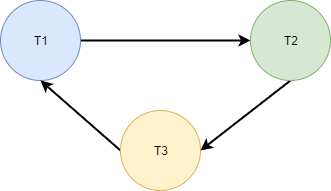
\includegraphics[width=0.4\linewidth]{img/deadlock}
		\caption{Példa holtpontra: $l_{1}(A); l_{2}(B); l_{3}(C); l_{1}(B); l_{2}(C); l_{3}(A)$}
		\label{fig:deadlock}
	\end{figure}
	
	\subsection*{Különböző zármódú zárolási rendszerek}
	
    \textbf{Probléma:} A $T$ tranzakciónak akkor is zárolnia kell az $X$ adatbáziselemet, ha csak olvasni akarja $X$-et, írni nem.
    \begin{itemize}
        \item Ha nem zárolnánk, akkor esetleg egy másik tranzakció azalatt írna $X$-be új értéket, mialatt $T$ aktív, ami nem sorba rendezhető viselkedést okoz.
        \item Másrészről pedig miért is ne olvashatná több tranzakció egyidejűleg $X$ értékét mindaddig, amíg egyiknek sincs engedélyezve, hogy írja.
    \end{itemize}

    \subsubsection*{Osztott és kizárólagos zárak}
    Mivel ugyanannak az adatbáziselemnek két olvasási művelete nem eredményez konfliktust, így ahhoz, hogy az olvasási műveleteket egy bizonyos sorrendbe soroljuk, nincs szükség zárolásra. \\
    Viszont szükséges azt az elemet is zárolni, amelyet olvasunk, mert ennek az elemnek az írását nem szabad közben megengednünk.\\
    Az íráshoz szükséges zár viszont "erősebb", mint az olvasáshoz szükséges zár, mivel ennek mind az olvasásokat, mind az írásokat meg kell akadályoznia. \\\\
    A legelterjedtebb zárolási séma két különböző zárat alkalmaz: az \emph{\textbf{osztott zár}}akat vagy olvasási zárakat, és a \emph{\textbf{kizárólagos zár}}akat vagy írási zárakat. \\\\
    Tetszőleges $X$ adatbáziselemet vagy egyszer lehet zárolni kizárólagosan, vagy akárhányszor lehet zárolni osztottan, ha még nincs kizárólagosan zárolva. \\
    Amikor írni akarjuk $X$-et, akkor $X$-en kizárólagos zárral kell rendelkeznünk, de ha csak olvasni akarjuk, akkor $X$-en akár osztott, akár kizárólagos zár megfelelő. \\\\
    Feltételezzük, hogy ha olvasni akarjuk $X$-et, de írni nem, akkor előnyben részesítjük az osztott zárolást.

    \begin{enumerate}
        \item Tranzakciók konzisztenciája: Nem írhatunk kizárólagos zár fenntartása nélkül, és nem olvashatunk valamilyen zár fenntartása nélkül.\\
        Minden zárolást követnie kell egy ugyanannak az elemnek a zárolását feloldó műveletnek.
        \item Tranzakciók kétfázisú zárolása: A zárolásoknak meg kell előzniük a zárak feloldását.
        \item Az ütemezések jogszerűsége: Egy elemet vagy egyetlen tranzakció zárol kizárólagosan, vagy több is zárolhatja osztottan, de a kettőegyszerre nem lehet.
    \end{enumerate}

	\paragraph*{Kompatibilitási mátrix}

    A kompatibilitási mátrix minden egyes zármódhoz rendelkezik egy sorral és egy oszloppal.\\

	\noindent A sorok egy másik tranzakció által az $X$ elemre már érvényes záraknak felelnek meg, az oszlopok pedig az $X$-re kért zármódoknak felelnek meg. \\

    \noindent A kompatiblitási mátrix használatának szabálya: Egy $A$ adatbáziselemre $C(=S \vee X)$ módú zárat akkor és csak akkor engedélyezhetünk, ha a táblázat minden olyan $R$ sorára, amelyre más tranzakció már zárolta $A$-t $R$ módban, a $C$ oszlopban ,,$\emph{Igen}$" szerepel.
	
	\begin{figure}[H]
		\centering
		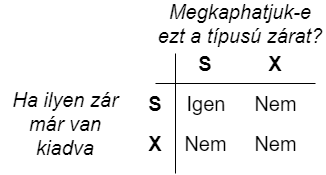
\includegraphics[width=0.40\linewidth]{img/kompmatrix}
		\caption{Az osztott ($S$) és kizárólagos ($X$) zárak kompatibilitási mátrixa.}
		\label{fig:kompmatrix}
	\end{figure}

    \paragraph*{Kompatibilitási mátrixok használata}
    \begin{enumerate}
        \item A mátrix alapján dönti el az ütemező, hogy egy ütemezés/zárkérés legális-e, illetve ez alapján várakoztatja a tranzakciókat. Minél több az ,,\emph{Igen}" a mátrixban, annál kevesebb lesz a várakoztatás.
        \item A mátrix alapján keletkező várakozásokhoz elkészített várakozási gráf segítségével az ütemező kezeli a holtpontot.
        \item A mátrix alapján készíti el az ütemező a megelőzési gráfot egy zárkérés-sorozathoz:
        \begin{itemize}
            \item a megelőzési gráf csúcsai trakzakciók és akkor van és $T_i$-ből $T_j$-be, ha van olyan $A$ adategység, amelyre az ütemezés során $Z_k$ zárat kért és kapott $T_i$, ezt engedte, majd
            \item ezután $A$-ra legközelebb $T_j$ kért és kapott olyan $Z_{s}$ zárat, hogy a mátrixban a $Z_k$ sor $Z_{s}$ oszlopában ,,\emph{Nem}" áll.\\
            Vagyis olyankor lesz él, ha a két zár nem kompatibilis egymással; nem mindegy a két művelet sorrendje\\
            \begin{center}
                $\ldots T_i:Z_k(A) \ldots T_i:UZ_k(A) \ldots T_j:Z_s(A)$\\
                $\uparrow \quad \text{ nem kompatibilis } \qquad \uparrow$
            \end{center}
        \end{itemize}
    \end{enumerate}
	
    \noindent A sorbarendezhetőséget a megelőzési gráf segítségével lehet eldönteni.\\

    \noindent \textbf{T:} Egy csak zárkéréseket és zárelengedéseket tartalmazó jogszerű ütemezés sorbarendezhető akkor és csak akkor, ha a kompatibilitási mátrix alapján felrajzolt megelőzési gráf nem tartalmaz irányított kört.
\end{document} 